\cleardoublepage

\chapter{Resultados experimentales}
\label{makereference7}

El sistema de optimización de baterías en el mercado eléctrico ha sido desplegado satisfactoriamente por lo menos en cuatro instalaciones, tres de topología híbrida y una de topología aislada, a lo largo de todo el país. El sistema mueve docenas de megavatios hora al día y genera millones de euros de ingreso al año.

El apartado de infraestructura operacional~\ref{makereference3} funciona continuamente obteniendo los datos de los sensores físicos de la instrumentación de campo y archivándolos en el sistema de información de planta. Los componentes del entorno de mercado~\ref{makereference4} obtienen la información del mercado, del sistema y meteorológica cada vez que cierra una sesión de mercado. La herramienta de modelización estructural~\ref{makereference5} optimiza la posición de las instalaciones con un periodo de correspondiente a la mínima diferencia entre la apertura de las sesiones de mercado. Finalmente, la consigna y control~\ref{makereference6} se comunica tanto a los activos energéticos como al mercado cada vez que se obtiene una nueva posición. El flujo se muestra en la figura~\ref{fig:flujo-procesamiento}.

\begin{figure}
  \centering
  \includegraphics[width=0.5\linewidth]{figures/flujo-procesamiento.png}
  \caption{Flujo de procesamiento de la información del sistema.}
  \label{fig:flujo-procesamiento}
\end{figure}

Con esto, para obtener los resultados experimentales, ha sido necesario realizar un trabajo previo de validación con el propósito de cerciorarse de los correctos resultados de las métricas operativas, es decir, investigar la rentabilidad del sistema.

Cabe destacar que, originalmente, la entidad con la que se realizó el despliegue del sistema apenas disponía de una herramienta altamente rudimentaria con un funcionamiento incorrecto únicamente enfocada en el arbitraje de topología aislada. Esto significa que, precisamente debido a la novedad de la tecnología de almacenamiento de energía en baterías, no se ha sido capaz de realizar comparaciones con soluciones similares debido a su nula existencia dentro de la entidad misma, por lo menos.

Aún así, se ha estudiado el rendimiento obtenido al sistema, analizando su uso no solo a lo largo del periodo de despliegue, sino realizando también simulaciones con datos de mercado y señales de la batería reales. Precisamente, facilitar el llamado \textit{backtesting} resulta ser una de las razones principales para el diseño de la arquitectura del sistema modular, con el sistema de control de planta de la infraestructura operacional y la base de datos del entorno de mercado.

De esta forma, cabe destacar que la métrica principal a analizar resulta siempre ser el beneficio obtenido en euros megavatio hora. La razón del uso de la unidad recae en el hecho de que no queremos vender la mayor cantidad de energía posible en todo momento, generando grandes beneficios, sino que lo que se desea maximizar, en cambio, es el \textit{spread}. Este, siendo la diferencia entre el precio al que se ha vendido y comprado el activo correspondiente, la energía en este caso, está sujeto a la unidades del mercado, el cual opera en euros por megavatio hora.

Con ello, la configuración operativa del sistema se mantiene en un \textit{spread} mínimo objetivo de 60 euros megavatio hora (\textit{€/MWh}) y una cantidad de ciclos máximos diarios de 1. El resto de parámetros operativos varían según la instalación controlada.

\section{Rentabilidad}
\label{makereference7.1}

Primeramente, es necesario conocer la información de rentabilidad para determinar si verdaderamente merece la pena la incorporación de sistemas de almacenamiento de energía en baterías en la red eléctrica, más allá de sus beneficios operativos.

Para ello, se debe conocer el coste de capital inicial de un sistema de almacenamiento de energía en baterías estándar de ion-litio, el cual puede ascender a las cifras incorporadas en la tabla~\ref{tab:rentabilidad-bess}.

Precisamente y asumiendo la configuración más favorable descrita en las secciones posteriores como~\ref{makereference7.4}, se observa que no son solo las baterías favorables para la diversificación de la red, sino que también generan beneficios por su cuenta gracias al aprovechamiento de la energía detallado en~\ref{makereference7.3}.

Junto a ello, cabe destacar que no se han tenido en cuenta las gigantescas ayudas económicas que las entidades energéticas reciben con el propósito de promover la energía renovable. Estas ayudas, en las que se incluyen las hibridaciones renovables con sistemas de almacenamiento, inclinan la balanza a favor de las baterías.

\begin{table}[ht]
  \centering
  \begin{tabular}{|c|p{7.5cm}|c|c|}
    \hline
    Tipo & Descripción         & Mnemónico & Prioridad\\
    \hline
    147  & Programa de consumo & M\_PC\_AA & Baja     \\
    \hline
  \end{tabular}
  \caption{Rentabilidad a lo largo del tiempo de un sistema de almacenamiento en baterías.}
  \label{tab:rentabilidad-bess}
\end{table}

\section{Operación manual}
\label{makereference7.2}

Pruebas empíricas en instalaciones de almacenamiento de energía en baterías en otras localizaciones en las que el sistema aún no ha sido desplegado, indican un enorme aumento en la eficiencia de la optimización.

Agentes de mercado indican tener que realizar sesiones de dos horas diarias con el único propósito de introducir las posiciones de mercado manualmente y comunicárselas a los operadores de telecomunicaciones para mandar las consignas\footnote{Aunque estas instalaciones no cuenten con el flujo desarrollado del sistema en el que las señales son comunicadas con el sistema de información de planta, existe un flujo alternativo a través de SCADA para operaciones manuales, como ya se ha descrito anteriormente}. Este trabajo de consignación manual es extremadamente propenso ha errores y completamente, o difícilmente, incapaz de aprovechar la temporalidad del proceso de optimización debido a la cantidad de combinaciones exponenciales de las posiciones de mercado cuanto más aumenta el horizonte de optimización. Situación similar a la dificultad del calculo manual del mejor movimiento en ajedrez.

La comparativa entre los resultados manuales contra el proceso del sistema desarrollado favorecen el uso de un sistema automatizado que no solo mejore de forma directa las ganancias generadas, sino que tenga en cuenta el entorno al completo y modifique su comportamiento según el mismo.

Sin disponer del sistema desarrollado, la estrategia de arbitraje más extendida entre los operadores de mercado que desvían dictar la posición de la batería se trata de la compra y venta directa de energía en los periodos valle y pico, respectivamente. Debido a la alta complejidad del arbitraje en los mercados intradiarios, los agentes de mercado únicamente definen la posición para el mercado diario de mayor liquidez.

Como se puede observar en la figura~\ref{fig:manual-vs-auto}, los dos principales problemas de la estrategia manual son el nulo aprovechamiento de los recursos híbridos de generación en las instalaciones que lo soportan, y la generación de desvíos ante falta de casaciones en el mercado diario que resultan en un perdida monetaria comparativamente significativa.

\begin{figure}
  \centering
  \includegraphics[width=0.5\linewidth]{figures/manual-vs-auto.png}
  \caption{Comparación del arbitraje entre la estrategia manual y la empleada por el sistema.}
  \label{fig:manual-vs-auto}
\end{figure}

\section{Configuración topológica}
\label{makereference7.3}

% TODO
% [fcr-price.jpg](https://dexterenergy.ai/news/bess-trading-the-case-for-cross-market-optimization/)
% Descenso promedio del precio de los mercados de ajuste por periodo.
% ``Aunque los mercados de ajuste todavía ofrezcan picos ocasionales que vale la pena aprovechar, las configuraciones aisladas ya no son suficientes como estrategia independiente''

Además, se han realizado análisis comparativos entre el rendimiento generado por cada una de las topologías, tanto aislada como híbrida, para determinar el aumento de beneficio que sistemas de optimización de baterías en el mercado eléctrico pueden aportar dependiendo de la configuración de la red.

Se observan las diferencias de beneficio comparativos de la figura~\ref{fig:aislado-vs-híbrido} a favor de las topologías híbridas (en su configuración más permisiva), siendo capaces de enrutar los flujos de carga desde diferentes fuentes. De esta forma, es entendible la tendencia de la industria de aumentar el número de instalaciones de colocación híbridas renovables y de almacenamiento simultáneamente.

La razón de la menor rentabilidad de la topología aislada viene dada porque su contraparte híbrida es capaz de cargar la batería en muchas ocasiones por precios nulos, mientras que la aislada siempre tiene que pagar por pasar por la red.

\begin{figure}
  \centering
  \includegraphics[width=0.5\linewidth]{figures/aislado-vs-híbrido.png}
  \caption{Resultados de arbitraje de las configuraciones topológicas de la infraestructura aislada e híbrida.}
  \label{fig:aislado-vs-híbrido}
\end{figure}

\section{Topología híbrida}
\label{makereference7.4}

Una vez comprobada la mejora del uso de instalaciones de topología híbrida, resulta interesante desglosar su operación en los tres modos de operación principales observados en la practica, el híbrido flexible, el híbrido con prioridad de carga renovable y el híbrido con carga aislada de la red.

Aunque las tres configuraciones híbridas sean capaces de aprovechar y rentabilizar la energía generada, es interesante comprobar cual de ellas es capaz de generar la mayor rentabilidad, con el propósito de priorizar su instalación.

\begin{figure}
  \centering
  \includegraphics[width=0.5\linewidth]{figures/híbrido-vs-híbrido.png}
  \caption{Comparativa del rendimiento de cada topología híbrida.}
  \label{fig:híbrido-vs-híbrido}
\end{figure}

En vista de los resultados obtenidos, de la figura  la configuración híbrida flexible es la que mayor rentabilidad genera, ya que es capaz de cargar tanto de la red como de la generación energética. Una de las claves de su mejora de rendimiento resultan los precios de mercado negativos. Estos, muy comunes en periodos de baja demanda, permiten obtener beneficio por comprar o cargar energía con el propósito de mantener la estabilidad de la red.

La configuración híbrida con prioridad de carga de generación, en cambio, no permite el aprovechamiento de los precios negativos ya que, irónicamente, debe priorizar la carga híbrida precisamente en los periodos de mayor generación, los cuales se corresponden con los de menor precio.

Por otro lado, la híbrida con carga aislada de la red es directamente incapaz de cargar de la red. Aunque con ella se asegure un \textit{lower bound} nulo del precio de compra, no se es capaz de aprovechar la generación al máximo debido a las restricciones de solamente poder cargar parte de la generación.

El integrador del sistema es capaz de modificar el funcionamiento físico \textit{on-site} de las instalaciones híbridas, incorporando el comportamiento flexible, para mejorar el rendimiento. Precisamente, tras el despliegue y obtención de resultados del sistema, la configuración topológica de una de las instalaciones se encuentra en proceso de modificación de híbrida con prioridad de carga renovable a híbrida flexible tras proponer el cambio.

\section{Arbitraje colaborativo}
\label{makereference7.5}

Finalmente, aunque la operación automática del sistema sea superior al control manual, eso no significa que los agentes de mercado no deban modificar su operación si piensan que es necesario para aumentar el beneficio.

Los agentes de mercado que operan el cuadro de mandos del sistema son capaces de detectar patrones externos que escapan al sistema. Uno de los fenómenos correspondientes más claro resulta ser la influencia de la temporalidad.

La temporalidad se aprecia en los precios del mercado, variando drásticamente según la demanda energética. En épocas calurosas y frías el precio aumenta, al igual que lo hace durante la semana, a diferencia del fin de semana. Con esto, es posible estudiar dicha temporalidad del mercado para atinar el ratio de ciclado de la batería: aumentarlo en las épocas más favorables y disminuirlo en las menos.

\begin{figure}
  \centering
  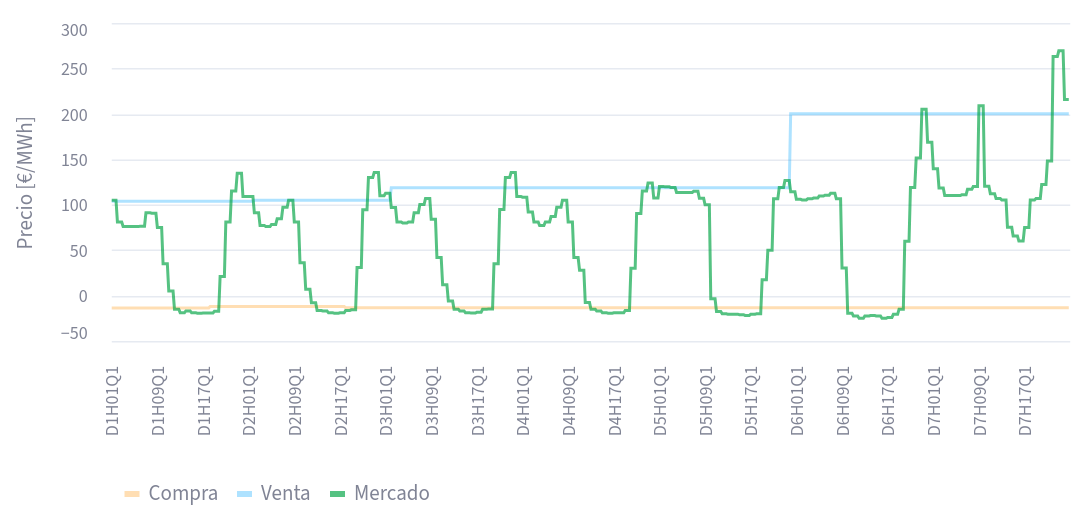
\includegraphics[width=0.5\linewidth]{figures/temporalidad-mercado.png}
  \caption{Variación del precio de mercado según el día de la semana.}
  \label{fig:temporalidad-mercado}
\end{figure}

La figura~\ref{fig:temporalidad-mercado}, que representa el ciclado energético ilimitado de una batería en diferentes condiciones de mercado a lo largo de la semana, muestra la variación de los momentos oportunos de arbitraje. Lamentablemente, el ciclado de los sistemas de almacenamiento de energía debe mantenerse limitado para mantener un ritmo predecible.

Un agente de mercado operando el cuadro de mandos del sistema, en cambio, puede conocer la temporalidad del mercado eléctrico y aprovechar los altibajos para indicarle al sistema un ritmo más alto o bajo del ciclado de las baterías.

Este modo de operación se conoce como arbitraje colaborativo y es recomendable para ajustar el comportamiento del sistema en busca del mayor beneficio, siendo en consecuencia el adoptado por la entidad de mercado.
